\section{Test}
In questa sezione vengono descritte le attività di testing, finalizzate alla verifica della qualità e dell’affidabilità del sistema.
\subsection{Test: CodeMR}
L’analisi statica conferma che OptiTour presenta una struttura solida. Il software risulta pulito e privo di componenti critici. L’assenza di “classi problematiche” dimostra che il codice è stato sviluppato con cura, mantenendo ogni modulo isolato e facilmente gestibile. Questo garantisce che il sistema sia semplice da manutenere e pronto per le iterazioni successive del progetto.

\begin{figure}[H]
    \centering
    % --- 2. COMPLESSITÀ ---
    \begin{minipage}[b]{0.32\textwidth}
        \centering
        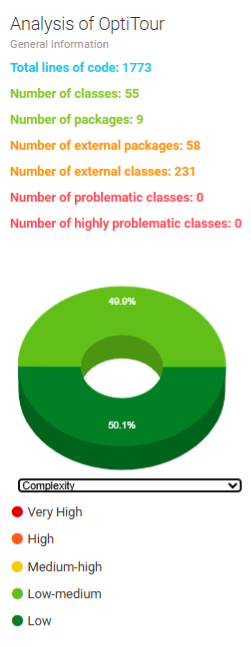
\includegraphics[width=\textwidth]{Iterazione1/Diagrammi/codeMR/complessità.png}
        \caption{Analisi della complessità.}
        \label{fig:IT1_Complexity_MVC}
    \end{minipage}
    \hfill
    % --- 3. ACCOPPIAMENTO ---
    \begin{minipage}[b]{0.32\textwidth}
        \centering
        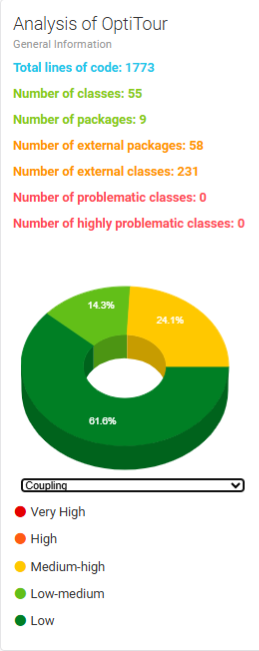
\includegraphics[width=\textwidth]{Iterazione1/Diagrammi/codeMR/Accoppiamento.png}
        \caption{Grado di accoppiamento.}
        \label{fig:IT1_Coupling_MVC}
    \end{minipage}
    \hfill
    % --- 4. COESIONE ---
    \begin{minipage}[b]{0.32\textwidth}
        \centering
        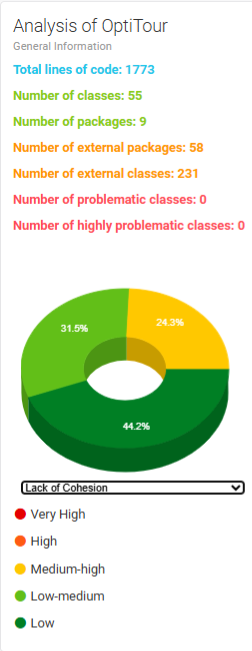
\includegraphics[width=\textwidth]{Iterazione1/Diagrammi/codeMR/MancanzaCoesione.png}
        \caption{Livello di coesione.}
        \label{fig:IT1_Cohesion_MVC}
    \end{minipage}
\end{figure}
% --- 1. STRUTTURA DEI PACKAGE ---
\begin{figure}[H]
    \centering
    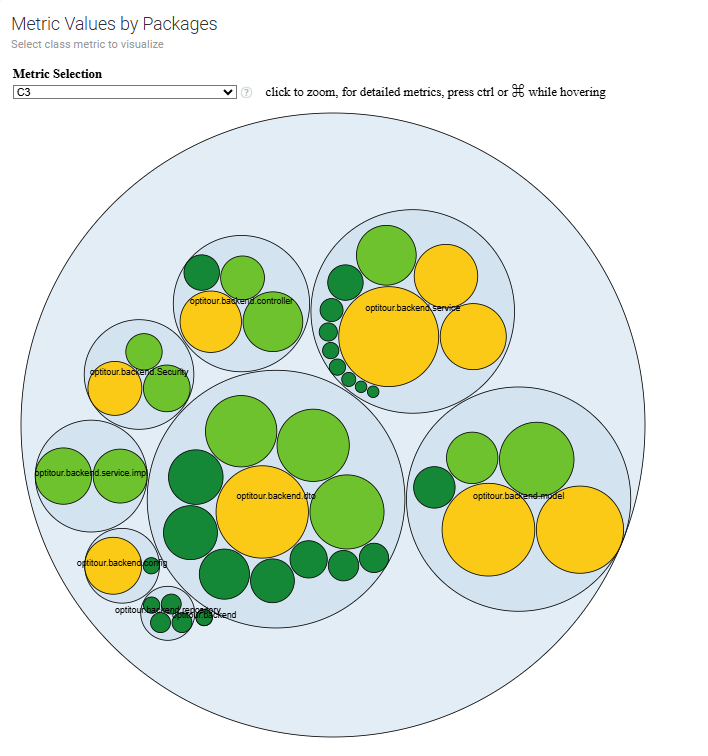
\includegraphics[width=0.8\textwidth]{Iterazione1/Diagrammi/codeMR/StrutturaPackage.png}
    \caption{Distribuzione dei componenti: organizzazione delle classi nei package Model, View/DTO, Service e Controller.}
    \label{fig:IT1_MVC_Structure}
\end{figure}


\newpage
\subsection{Test: Junit}